%!TEX root = kotov.tex
\section{Task 2}
\begin{task}
    Дано дерево $T = \braket{V,E}$. За $\O(V + E)$ вычислить для каждого ребра, сколько простых путей проходит через него.
\end{task}

\begin{solution}
    Так как исходный граф --- дерево, то любое ребро в нем является мостом, то есть если мы разобьем наш граф на две доли по этому ребру, то оно будет единственным ребром, соединяющим эти доли.
    Будем это эксплуатировать: рассмотрим какие-то две доли дерева (назовем их ``кексы'', потому что очень похожи и так чуть-чуть повеселее).
    \begin{figure}[H]
        \centering
        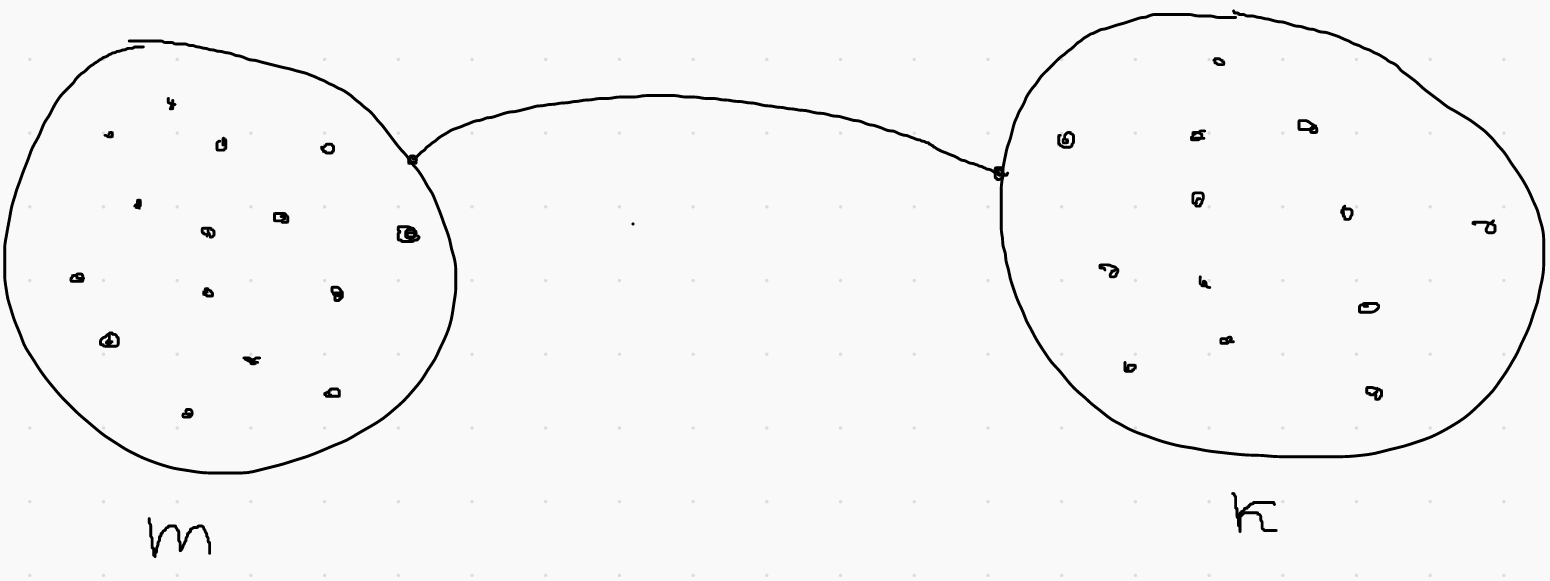
\includegraphics[width=0.7\textwidth]{pics/cake.png}
        \caption{Два кекса. Количество вершин слева равно $m$, справа --- $k$, суммарно $n$}
    \end{figure}
    Тогда, количество путей, содержащих рассматриваемый мост равно $mn$, так как мы из любой вершины слева может достигнуть любую вершину справа.
    Теперь останется только напечь таких кексов, но это просто: можем для каждой вершины $v$ чем-то похожим на \texttt{dfs} посчитать количество вершин в поддереве с корнем $v$.
    
    Формально это заняло бы $\O(V+E)$, а потом для каждого ребра, как для моста, выпекать два кекса и считать за $\O(1)$ количество путей, так как количество элементов для левого кекса можно взять из корня соответствующего поддерева, а количество элементов в правом кексе есть $n -\#\text{элементов в левом кексе}$.
    \begin{figure}[H]
        \centering
        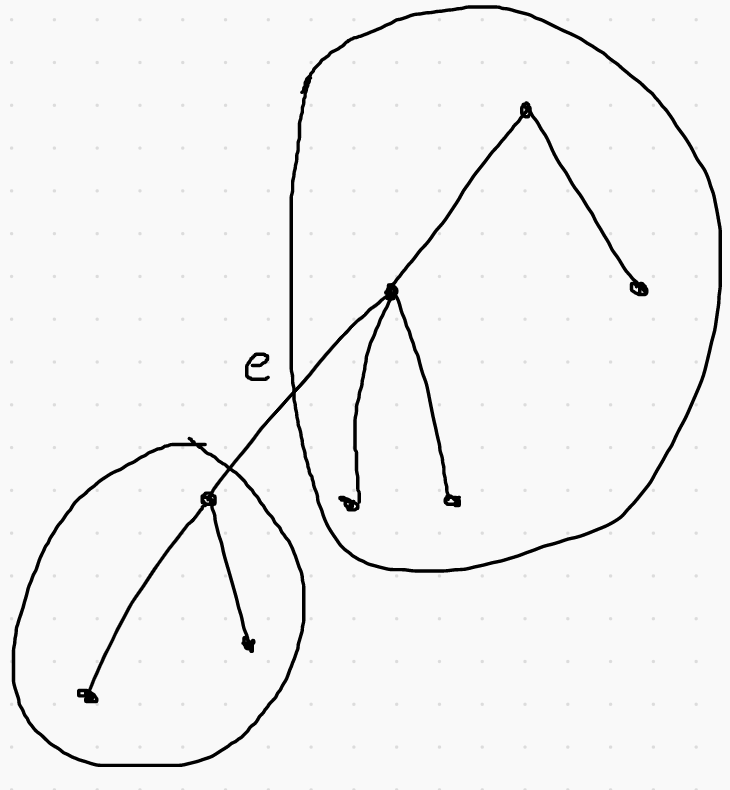
\includegraphics[width=0.4\textwidth]{pics/cake_tree.png}
        \caption{Поясняющая картинка к дереву и кексам.}
    \end{figure}
    \begin{remark}
        Можно заметить, что в дереве, количество вершин $\sim$ количество ребер, тогда реально сложность будет $\O(E)$.
    \end{remark}
\end{solution}

\begin{upd}
    Как именно мы считаем количество вершин в поддереве с корнем в v? Это можно сделать следующим образом: мы обновим значение количества вершин в поддереве как сумму вершин в детях плюс одну за сам корень, предположим, что мы поиском в глубину спустились до листа, когда начинаем из него выходить (подниматься наверх) мы обновляем количество вершин в поддереве этого листа (очевидно, что там всего $1$ вершина), если у родителя этого листа есть еще дети, то мы спускаемся в них. Для простоты рассмотрим пример, где у родителя всего два листа:
    \begin{enumerate}
        \item мы спустились в первый лист, посчитали количество вершин в поддереве этого листа, как на корне (то есть записали для него $1$).
        \item вернулись к родителю, увидели второго ребенка
        \item спустились во второго ребенка, посчитали количество вершин бла-бла-бла, записали $1$.
        \item вернулись опять к этому родителю, увидели, что больше детей тут нет и надо подниматься выше
        \item обновили значение у этого родителя (сумма значений в детях $+1$ за себя, то есть в этом примере будет записана $3$ в эту вершину)
        \item продолжаем такую процедуру выше (надеюсь, я понятно переложил мысль в слова).
    \end{enumerate}
\end{upd}